\chapter{Method}
\label{chapter:secorder}
This chapter describes the experimental methods and technical processes employed in this study and elaborates on how indeterminacy analysis can enhance the predictive capability and stability of the proposed models. The primary objective of this chapter is to propose an indeterminacy judgment method that predicts outcomes by introducing multiple instances of varying noise to the same sample, thereby quantifying indeterminacy and optimizing classification decisions accordingly.

The methodology presented in this chapter is structured into three main components. First, Section 3.1 outlines the data preprocessing techniques, the design of the machine learning models, and the training process used in this study. Second, Section 3.2 explains how multiple passes through perturbed samples are used to analyze sample indeterminacy and compute the probability means and variances of the predictions. Finally, Section 3.3 demonstrates how classification decisions are made based on the indeterminacy evaluation results, categorizing samples into "determinate" (True/False) or "indeterminate" (Indeterminate) classes.

In modern clinical applications, there is an increasing demand for diagnostic precision and robustness, particularly in the early detection of vascular access dysfunction. Traditional diagnostic approaches often rely on fixed blood flow thresholds, which can lead to misdiagnoses or missed diagnoses due to fluctuations in individual values. The primary goal of this study is to address this problem by introducing the concept of indeterminacy analysis, which adjusts classification decisions to ensure that the system provides more cautious diagnostic outcomes for ambiguous samples. The framework proposed in this chapter effectively addresses the limitations of traditional diagnostic methods, enabling the system to classify clear samples accurately while also offering indeterminacy evaluations for borderline cases, thereby enhancing its utility in clinical applications.

\begin{comment} 
Section ordering in \textit{thesis.cls} is:
\begin{itemize}
\item Chapter (shown in \textbf{Table of Contents})
\item Section (shown in \textbf{Table of Contents})
\item Subsection (shown in \textbf{Table of Contents})
\item Paragraph
\item Subparagraph
\end{itemize}
DONOT use \textbackslash subsubsection, it is not supported in \textit{thesis.cls}.
It is replaced by \textbackslash paragraph.
\end{comment}

\section{Model Architecture}
In this chapter, we introduce the proposed Indeterminacy Classification Model designed to classify samples, as illustrated in Figure 3.1.

\begin{figure}[H]
    \centering
    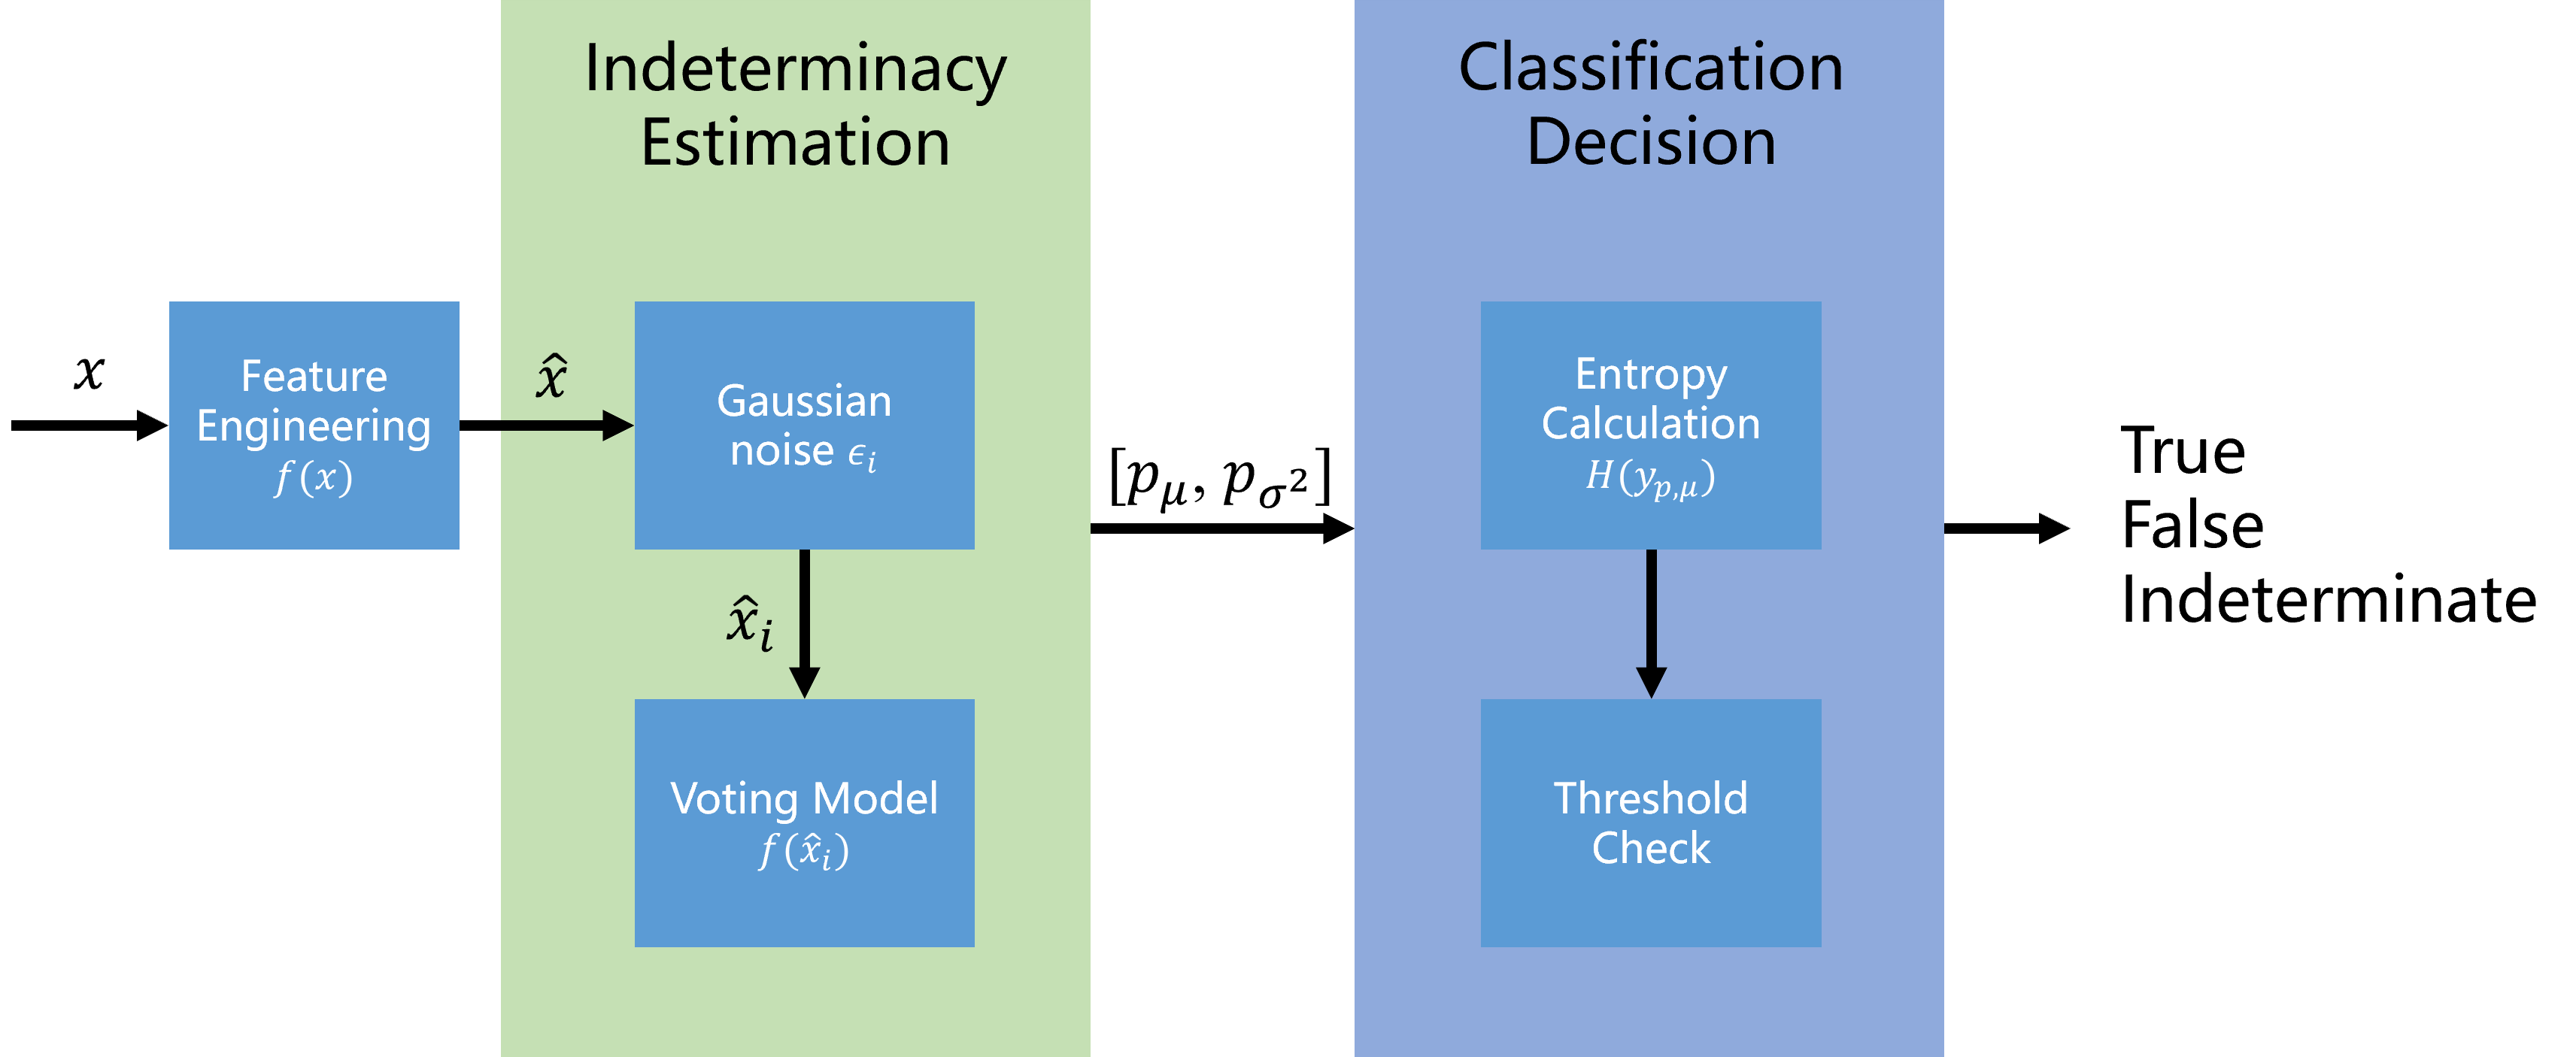
\includegraphics[width=1\linewidth]{figures/model_architecture.png}
    \caption{Indeterminacy Classification Model}
    \label{fig:enter-label}
\end{figure}

The structured dataset underwent preprocessing steps, which included removing redundant information, feature creation, and aligning the data. These steps ensure that the dataset is clean and suitable for training machine learning models. For a detailed explanation of the preprocessing steps, please refer to Chapter 4.2.

The models utilized in this study are tree-based machine learning classifiers, specifically:

\begin{itemize}
    \item \textbf{Decision Tree}: A fast and interpretable model; however, it is prone to overfitting when applied to high-dimensional data.
    \item \textbf{Random Forest}: An ensemble of decision trees that effectively reduces model variance and improves prediction stability.
    \item \textbf{XGBoost}: A gradient boosting framework renowned for its computational efficiency and strong classification performance, particularly in imbalanced datasets.
\end{itemize}

To leverage the strengths of these models, we implemented a weighted soft voting strategy, combining the prediction probabilities from each model. This approach allows the ensemble to capture diverse perspectives from the individual classifiers. Furthermore, to address the imbalance between positive and negative samples, we adjusted the \texttt{scale\_pos\_weight} parameter in XGBoost, ensuring that the model assigns appropriate importance to minority class samples. All models were trained and evaluated using K-fold cross-validation, which ensures robust and reliable performance.

After constructing the soft voting model, it was integrated into the Multipass Indeterminacy Estimation Method and the Indeterminate-Aware Data Classification process. These methods enhance the classification framework by quantifying and addressing indeterminacy, further improving the model's applicability in complex scenarios.

\section{Multipass Indeterminacy Estimation Method}% Algorithm
To quantify the indeterminacy of each sample, we propose the Multipass Indeterminacy Estimation Method. The key idea is to generate multiple perturbed versions of each sample by adding Gaussian noise $\epsilon=N(\mu,\sigma^2)$. Each perturbed version of the sample is then passed through the weighted soft voting classifier, which predicts the probabilities for True and False. The predicted probabilities for True and False across all perturbed versions are then aggregated to calculate their respective means ($p_{u}$) and variances ($p_{\sigma^2}$). This process is repeated for each sample individually.

The main steps of this method are:
\begin{enumerate}
  \item \textbf{Perturbed Sample Generation}: Adding Gaussian noise to the input features to simulate data indeterminacy, creating multiple perturbed versions of the sample.
  \item \textbf{Multi-Model Prediction}: Passing each perturbed version through the soft voting classifier, which integrates predictions from Decision Tree, Random Forest, and XGBoost to generate probabilities for $True$ and $False$.
  \item \textbf{Probability Mean and Variance Calculation}: Aggregating the predicted probabilities for True and False across all perturbed versions by calculating their respective means ($p_{u}$) and variances ($p_{\sigma^2}$).
\end{enumerate}

The use of multiple perturbed versions of a sample considers the fact that a patient’s current blood flow rate is not fixed but continuously fluctuating. By generating multiple perturbed inputs representing variations in blood flow rates for the same patient, the model can simulate real-world conditions. This approach enables the model to provide more confident and robust predictions under varying circumstances.

\begin{algorithm}[H]
\caption{Multipass Indeterminacy Estimation}
\label{alg:Training}
\begin{algorithmic}[1]
\Statex \textbf{Input:} 
\Statex \hspace{1em} \(\hat{x}\): Input sample, \(\mu\): Noise mean, \(\sigma^2\): Noise variance
\Statex \hspace{1em} \(W=[w_{1},w_{2},w_{3}]\): Weight of estimator, \(n\): Number of estimation times
\Statex \hspace{1em} \(Estimators\): \([Decision Tree, Random Forest, XGBoost]\)
\Statex \textbf{Output:} 
\Statex \hspace{1em} \(p_{\mu}\): Mean of probability, \(p_{\sigma^2}\): Variance of probability
\Statex \textbf{Initialize:}
\Statex \hspace{1em} $\hat{P}=[\hspace{1em}]$
\State \textbf{for} estimate \(i\) from \(1\) to \(n\) \textbf{do}
\State \hspace{1em} \(\epsilon_{i} \sim N(\mu,\sigma^2)\) 
\State \hspace{1em} \(\hat{x_{i}} \leftarrow \hat{x} + \epsilon_{i} \)
\State \hspace{1em} \(P_{y_{i}} = [\hspace{1em}]\)
\State \hspace{1em} \textbf{for} \(clf\) in \(Estimators\) \textbf{do}
\State \hspace{2em} \(v_{clf} = VotingClassifier(clf, voting = 'soft')\)
\State \hspace{2em} \(p_{y_{i}, clf} = v_{clf}.PredictProb(\hat{x_{i}})\) \(\# p=[p_{T},p_{F}]\)
\State \hspace{2em} Append \(p_{y_{i}, clf}\) to \(P_{y_{i}}\)
\State \hspace{1em} \textbf{end}
\State \hspace{1em} \(\hat{p_{i}}=average(P_{y_{i}}, W)\)
\State \hspace{1em} Append \(P_{y_{i}}\) to \(\hat{P}\)
\State \textbf{end}
\State \(p_{\mu}=mean(\hat{P})\) \(\# p_{\mu}=[p_{T,\mu},p_{F,\mu}]\)
\State \(p_{\sigma^2}=variance(\hat{P})\) \(\# p_{\sigma^2}=[p_{T,\sigma^2},p_{F,\sigma^2}]\)
\State return \(p_{\mu}\), \(p_{\sigma^2}\)
\end{algorithmic}
\end{algorithm}

Algorithm 3.1 demonstrates the process of performing Multipass Indeterminacy Estimation. This method involves iteratively sampling noise \(\epsilon\) from a standard Gaussian distribution to simulate variability. The noise \(\epsilon\) is then combined with the original blood flow rate of the sample, producing perturbed blood flow rates. These perturbed values are subsequently passed through an ensemble learning model with a soft voting mechanism, where the predictions from individual models are weighted and averaged to generate probability distributions for the perturbed blood flow rates. Finally, the mean and variance of these probability distributions are calculated to determine the likelihood of whether the sample requires surgical intervention. This approach quantifies the indeterminacy inherent in the prediction, ensuring robust and confident decision-making.

After processing all perturbed versions of a sample, the method moves on to the next sample, repeating the process until all samples are evaluated. This approach effectively captures data indeterminacy and provides robust and reliable prediction outputs.

\section{Indeterminate-Aware Data Classification}% Algorithm
Based on the results of the multipass method, we propose an Indeterminate-Aware Data Classification strategy. This method classifies samples into three categories: $True$, $False$, and $Indeterminate$.

Algorithm 3.2 demonstrates classifying which data are determinate or which data are indeterminate. This method is implemented in two steps. First, the information entropy $H(y_{p,u})$ of the probability distribution is calculated to quantify its uniformity. If the entropy exceeds a predefined threshold $\theta_{u}$, the sample is classified as $Indeterminate$, indicating insufficient confidence in the prediction.

\begin{equation}
H(y_p,\mu) = -(p_{T,\mu}\log p_{T,\mu}+p_{F,\mu}\log p_{F,\mu})
\end{equation}

Second, for samples with entropy below the threshold, their probability distributions' means and variances are further evaluated to classify them as $True$ or $False$. Samples with minimal mean differences and large variances are reclassified as $Indeterminate$ to reduce misclassification risks.

The classification decisions in Indeterminate-Aware Data Classification are guided by the probability means \(p_{T,\mu},p_{F,\mu}\) and variances \(p_{T,\sigma^2},p_{F,\sigma^2}\) of the predicted probabilities for "True" and "False." These two equations are used to classify a sample as "True" or "False" while accounting for indeterminacy in the predictions.

\subsection{Condition True}

This equation determines whether the sample is classified as "True." It includes two conditions:

\begin{equation}
p_{T,\mu} > p_{F,\mu} \textbf{ and } p_{T,\mu} - \sqrt{p_{T,\sigma^2}} > p_{F,\mu} + \sqrt{p_{F,\sigma^2}}
\end{equation}

\begin{itemize}
    \item \(p_{T,\mu}\) > \(p_{F,\mu}\): The mean probability of "True" is greater than that of "False."
    \item \(p_{T,\mu} - \sqrt{p_{T,\sigma^2}}\) > \( p_{F,\mu} + \sqrt{p_{F,\sigma^2}}\): This ensures that even after accounting for the variability (as represented by the standard deviation), the confidence in "True" exceeds that of "False." The subtraction and addition of the square root of variances serve to introduce a conservative buffer for decision-making.
\end{itemize}

Only when both conditions are met does the sample get classified as "True." This approach reduces the risk of misclassification due to overlapping confidence intervals.

\subsection{Condition False}

This equation mirrors Equation 3.2 but applies to the classification of "False." Similarly, it requires:

\begin{itemize}
    \item \(p_{F,\mu}\) > \(p_{T,\mu}\): The mean probability of "False" is greater than that of "True."
    \item \(p_{F,\mu} - \sqrt{p_{F,\sigma^2}}\) > \( p_{T,\mu} + \sqrt{p_{T,\sigma^2}}\): After accounting for variability, the confidence in "False" must still dominate over "True."
\end{itemize}

\begin{equation}
p_{F,\mu} > p_{T,\mu} \textbf{ and } p_{F,\mu} - \sqrt{p_{F,\sigma^2}} > p_{T,\mu} + \sqrt{p_{T,\sigma^2}}
\end{equation}

When both conditions are satisfied, the sample is classified as "False." Like the previous equation, this ensures a robust classification by considering prediction indeterminacy.

\begin{algorithm}[H]
\caption{Indeterminate-Aware data classification}
\label{alg:Training}
\begin{algorithmic}[1]
\Statex \textbf{Input:} 
\Statex \hspace{1em} \(p_{\mu}\): Mean of probability,which is \([p_{T,\mu},p_{F,\mu}]\)
\Statex \hspace{1em} \(p_{\sigma^2}\): Variance of probability,which is \([p_{T,\sigma^2},p_{F,\sigma^2}]\)
\Statex \hspace{1em} \(\theta_{\mu}\): Threshold used to determine output of indeterminacy
\Statex \textbf{Output:} 
\Statex \hspace{1em} \("True", "False" or "Indeterminate"\)
\State \(H(y_p,\mu) \leftarrow -(p_{T,\mu}\log p_{T,\mu}+p_{F,\mu}\log p_{F,\mu})\) 
\State \textbf{if} \(H(y_p,\mu)\) > \(\theta_{\mu}\) \textbf{then}
\State \hspace{1em} \textbf{return} \("Indeterminate"\)
\State \textbf{else}
\State \hspace{1em} \textbf{if} \(p_{T,\mu}\) > \(p_{F,\mu}\) \textbf{and} \(p_{T,\mu} - \sqrt{p_{T,\sigma^2}}\) > \( p_{F,\mu} + \sqrt{p_{F,\sigma^2}}\) \textbf{then}
\State \hspace{2em} \textbf{return} \("True"\)
\State \hspace{1em} \textbf{else if} \(p_{F,\mu}\) > \(p_{T,\mu}\) \textbf{and} \(p_{F,\mu} - \sqrt{p_{F,\sigma^2}}\) > \( p_{T,\mu} + \sqrt{p_{T,\sigma^2}}\) \textbf{then}
\State \hspace{2em} \textbf{return} \("False"\)
\State \hspace{1em} \textbf{else}
\State \hspace{2em} \textbf{return} \("Indeterminate"\)
\end{algorithmic}
\end{algorithm}

This classification strategy effectively handles boundary samples, minimizing erroneous predictions while providing higher confidence in clinical decision-making.

%\subsection{Subsection}
